\chapter{Methodology}\singlespacing % Main chapter title

\label{Chapter3} % Change X to a consecutive number; for referencing this chapter elsewhere, use \ref{ChapterX}

\lhead{Chapter 3. \emph{Methodology}} % Change X to a consecutive number; this is for the header on each page - perhaps a shortened title

%----------------------------------------------------------------------------------------
%	SECTION 1
%----------------------------------------------------------------------------------------

\section{Definition of Neuron}

In the context of multi layer perceptrons (MLPs) in large language models (LLMs), a \textit{neuron} refers to a unit of computation within the MLP module. Specifically, consider the $i^\text{th}$ layer of a Transformer architecture, where the input is a hidden state vector $\mathbf{H}^{i-1} \in \mathbb{R}^{T \times d}$, derived from the previous layer.

\textbf{Hidden State Representation}:  The output of the multi-head self-attention (MHA) mechanism serves as input to the MLP and is given as:
\begin{equation}
\hat{\mathbf{H}}^i = \text{Attn}(\mathbf{H}^{i-1}\mathbf{W}_q^i, \mathbf{H}^{i-1}\mathbf{W}_k^i, \mathbf{H}^{i-1}\mathbf{W}_v^i) \cdot \mathbf{W}_o^i,
\end{equation}
where $\mathbf{W}_q^i, \mathbf{W}_k^i, \mathbf{W}_v^i, \mathbf{W}_o^i \in \mathbb{R}^{d \times d}$ are the trainable parameters of the self-attention module, and $\text{Attn}(\cdot)$ denotes the scaled dot-product attention operation.

\textbf{MLP Transformation}: The MLP module takes $\hat{\mathbf{H}}^i$ as input and transforms it as follows:
\begin{equation}
\mathbf{h}^i = \text{act\_fn}(\hat{\mathbf{H}}^i \mathbf{W}_1^i) \cdot \mathbf{W}_2^i,
\end{equation}
where $\mathbf{W}_1^i \in \mathbb{R}^{d \times 4d}$ and $\mathbf{W}_2^i \in \mathbb{R}^{4d \times d}$ are learnable projection matrices, and $\text{act\_fn}(\cdot)$ represents a non-linear activation function such as GELU or SiLU.

\textbf{Neuron}: Within the MLP, the $j^\text{th}$ neuron of the $i^\text{th}$ layer corresponds to the $j^\text{th}$ row of the intermediate activation matrix:
\begin{equation}
\mathbf{h}_j^i = \text{act\_fn}((\hat{\mathbf{H}}^i \mathbf{W}_1^i)_j),
\end{equation}
where $(\hat{\mathbf{H}}^i \mathbf{W}_1^i)_j$ represents the pre-activation value of the $j^\text{th}$ neuron.

\textbf{Generalized Neuron Formulation}: Recent architectures such as LLaMA [\cite{grattafiori2024llama}] utilize Gated Linear Units (GLU) to enhance MLP performance, modifying the MLP computation as:
\begin{equation}
\mathbf{h}^i = [ \text{act\_fn}(\hat{\mathbf{H}}^i \mathbf{W}_1^i) \otimes (\hat{\mathbf{H}}^i \mathbf{W}_3^i) ] \cdot \mathbf{W}_2^i,
\end{equation}
where $\mathbf{W}_3^i \in \mathbb{R}^{d \times 4d}$ is an additional projection matrix, and $\otimes$ denotes element-wise multiplication. This formulation introduces gating to the MLP, allowing for more expressive transformations. Figure~\ref{fig:mlp} shows the architecture of the MLP module.

\begin{figure}[ht]
	\centering
	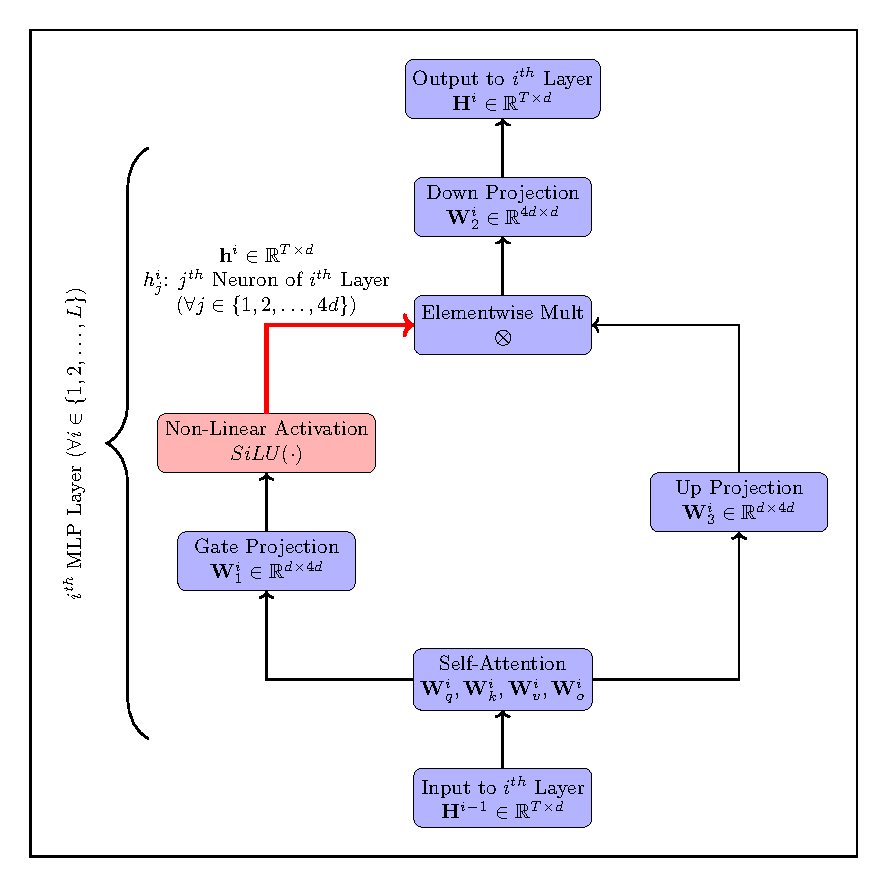
\includegraphics[width=\textwidth]{Chapters/Chapter_3/mlp.pdf} % Adjust the width as needed
	\caption{Architecture of MLP module in LLaMA model}
	\label{fig:mlp}
\end{figure}

\section{Dataset for Neuron Identification}

For the purpose of identifying language-specific neurons, we utilize a subset of the Wikipedia dataset spanning 15 languages:
\[
\text{\{en, fr, es, vi, id, ja, zh, bn, hi, ta, te, mr, ur, kn, ml, pa\}}.
\]
Each language's dataset is preprocessed and passed through pretrained large language models (LLMs). The activations are then collected from the MLP modules of the models.

\textbf{Dataset Description:}
The Wikipedia dataset [\cite{wikidump}] for each language contains a sequence of tokenized text data. Each tokenized sequence has a maximum length of $T_{\max} = 512$. For every sequence, we compute the activations from the MLP module, followed by averaging the activations at each neuron position across all sequences. This provides a language-specific profile for every neuron $(i, j)$ in the model.

\textbf{Activation Collection:} 
Given a pretrained LLM, let the MLP activation for the $i^\text{th}$ layer and the $j^\text{th}$ neuron in a specific language be represented by $h_{i,j}^t \in \mathbb{R}$, where $t$ indexes the token positions in a sequence of length $T$. The average activation of a neuron across all token positions for a given sequence is computed as:
\begin{equation}
\bar{h}_{i,j} = \frac{1}{T} \sum_{t=1}^{T} h_{i,j}^t,
\end{equation}
where $h_{i,j}^t$ is the neuron activation corresponding to the $t^\text{th}$ token.

\textbf{Language-Specific Activations:}
For each language $l$ in the dataset, we compute the average activation of each neuron $(i, j)$ over all sequences $S_l$ in the dataset:
\begin{equation}
h_{i,j}^l = \frac{1}{|S_l|} \sum_{s \in S_l} \bar{h}_{i,j}^{(s)},
\end{equation}
where $h_{i,j}^l$ represents the average activation of the $j^\text{th}$ neuron in the $i^\text{th}$ layer for language $l$, and $|S_l|$ denotes the number of sequences for language $l$.


\section{Statistics of Neuron Activation}

The statistics of neuron activation are precomputed to analyze language-specific patterns in the MLP layers of the pretrained large language models (LLMs). These statistics include mean, standard deviation, and quantiles (e.g., 5th, 10th, 25th, 50th, 75th, 90th, and 95th percentiles) of the neuron activations for each language in the dataset. The computations are performed across all layers and neurons within the MLP modules.

\textbf{Activation Mean and Standard Deviation:} The mean activation of a neuron $(i, j)$ in the $t^\text{th}$ token position is computed as:
\begin{equation}
\mu_{i,j} = \frac{1}{T} \sum_{t=1}^T h_{i,j}^t,
\end{equation}
where $h_{i,j}^t$ is the activation of the $(i,j)$ neuron for the $t^\text{th}$ token, and $T$ is the total number of tokens in a sequence. Similarly, the standard deviation of the activations is calculated as:
\begin{equation}
\sigma_{i,j} = \sqrt{\frac{1}{T} \sum_{t=1}^T (h_{i,j}^t - \mu_{i,j})^2}.
\end{equation}

\textbf{Quantiles of Activation:} Quantile-based statistics provide insights into the distribution of activations for each neuron. The $q$-quantile activation value, denoted as $P_q$, is defined as:
\begin{equation}
P_q(h_{i,j}) = \inf \left\{x \in \mathbb{R} : F_{h_{i,j}}(x) \geq q \right\},
\end{equation}
where $F_{h_{i,j}}(x)$ is the cumulative distribution function (CDF) of the activations for neuron $(i, j)$. Commonly computed quantiles include:
\[
P_{50}, \, P_{75}, \, P_{90}, \, P_{95}, \, P_{25}, \, P_{10}, \, P_{5}.
\]

\textbf{Language-Specific Aggregation:} For a given language $l$ and all sequences in the dataset, the mean and other statistics are aggregated across all token positions and batches. Let $S_l$ denote the set of sequences for language $l$, and $B$ represent the batch size. The aggregated mean activation for neuron $(i, j)$ is computed as:
\begin{equation}
\bar{\mu}_{i,j}^l = \frac{1}{|S_l|} \sum_{b=1}^B \sum_{s \in S_l} \mu_{i,j}^{(s,b)},
\end{equation}
where $\mu_{i,j}^{(s,b)}$ is the mean activation of neuron $(i, j)$ for the $s^\text{th}$ sequence in the $b^\text{th}$ batch.

\section {Methods for Neuron Identification}

\subsection{LAPE}

Language Activation Probability Entropy (LAPE) [\cite{tang2024languagespecific}] is a method designed to identify neurons that exhibit language-specific behavior across multiple languages. This metric quantifies the entropy of normalized activation probabilities for each neuron across the given set of languages.

\textbf{Step 1: Compute Activation Probabilities.} 
For a pretrained large language model with $L$ layers and $4d$ neurons per layer, the activation of a neuron $(i, j)$ in response to a sequence $X^l \in \mathbb{R}^{N \times T}$ (where $N$ is the number of sequences, and $T$ is the number of tokens per sequence) for a language $l$ is denoted as $h_{i,j}^l$. The unnormalized activation probability for neuron $(i, j)$ is given by:
\begin{equation}
	p_{i,j}^l = \mathbb{E}\left[\mathbb{I}\left(h_{i,j}^l > 0\right)\right],
\end{equation}
where $\mathbb{I}$ is the indicator function that returns $1$ if the activation $h_{i,j}^l$ is greater than zero, and $0$ otherwise. The expectation is computed over all tokens in all sequences for language $l$.

\textbf{Step 2: Normalize Activation Probabilities.} 
The normalized activation probability is computed across $k$ languages to ensure a valid probability distribution:
\begin{equation}
	P_{i,j}^l = \frac{p_{i,j}^l}{\sum_{l=1}^k p_{i,j}^l}, \quad \forall i \in \{1, \dots, L\}, \, \forall j \in \{1, \dots, 4d\}.
\end{equation}

\textbf{Step 3: Compute Language Activation Probability Entropy.} 
The entropy of the normalized activation probabilities for each neuron $(i, j)$ is computed as:
\begin{equation}
	\text{LAPE}(i, j) = - \sum_{l=1}^k P_{i,j}^l \log P_{i,j}^l, \quad \forall i \in \{1, \dots, L\}, \, \forall j \in \{1, \dots, 4d\}.
\end{equation}
This measures the uncertainty in the activation distribution of a neuron across the $k$ languages. Figure~\ref{fig:lape} shows the procedure of computing LAPE for a neuron.

\textbf{Step 4: Apply Threshold and Select Neurons.} 
To identify neurons with significant language-specific behavior, a threshold is defined based on the $95^\text{th}$ percentile of the unnormalized activation probabilities:
\begin{equation}
	\text{Threshold} = \text{Quantile}_{0.95}\left(p_{i,j}^l \, | \, \forall i, j, l\right).
\end{equation}
A neuron $(i, j)$ is considered for language-specific analysis only if:
\begin{equation}
	\exists l \in \{1, \dots, k\} \, \text{such that} \, p_{i,j}^l > \text{Threshold}.
\end{equation}

\textbf{Step 5: Select Top Neurons Based on LAPE.} 
Only 1\% neurons with the lowest LAPE values are selected for language-specific analysis, where $m$ is defined as:
\begin{equation}
	m = \frac{1 \times 4d \times L}{100}.
\end{equation}
The top \(m\) neurons are identified by sorting the LAPE values and selecting the indices of the \(m\) smallest values:
\begin{equation}
	\text{Top}_m(\text{Lang\_Set}) = \text{argsort\_ascending}_m \left\{\text{LAPE}(i,j) \,|\, \forall i, j, \exists l \,\, s.t. \,\,  p_{i,j}^l > \text{Threshold} \right\}.
\end{equation}
This ensures that only the most language-specific neurons are retained for further interpretation. 

\textbf{Step 6: Identify Language-Specific Neuron Sets.} 
For each neuron $(i, j)$ in the selected set, the language-specific set is defined as:
\begin{equation}
	\text{Lang\_Spec\_Set}(i, j) = \left\{ l \, | \, p_{i,j}^l > \text{Threshold}, (i,j) \in \text{Lang\_Set} \right\}.
\end{equation}

A neuron is considered specific to a subset of languages if:
\begin{equation}
	\text{Lang\_Spec\_Set}(i, j) \subseteq \{1, 2, \dots, k\}.
\end{equation}

\begin{figure}[ht]
	\centering
	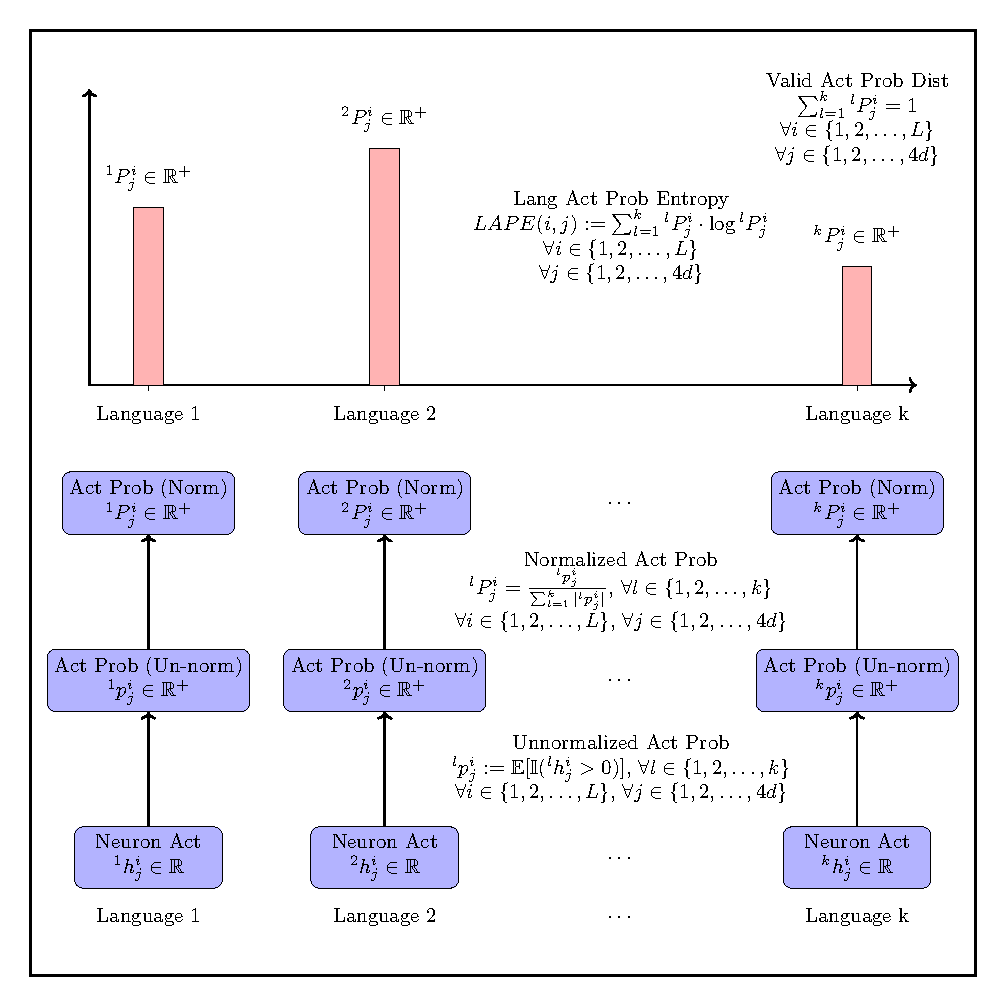
\includegraphics[width=\textwidth]{Chapters/Chapter_3/lape.pdf} % Adjust the width as needed
	\caption{Procedure of computing LAPE for a neuron.}
	\label{fig:lape}
\end{figure}

\subsection{Activation Based Methods}

\textbf{Absolute Activation:} The absolute activation metric measures the mean absolute activation of each neuron \((i, j)\) in the \(i^\text{th}\) layer across all tokens in a sequence for a language \(l\). This is computed as:
\begin{equation}
	r_{i,j}^l = \mathbb{E}\left[\left| h_{i,j}^l \right|\right],
\end{equation}
where \( h_{i,j}^l \) is the activation of neuron \((i, j)\) for language \(l\), and the expectation is taken over all tokens and sequences. This metric identifies neurons with consistently high absolute activations, which are indicative of their overall importance in representing language features.

\textbf{Activation Probability Zero:} The activation probability zero metric measures the fraction of times a neuron \((i, j)\) has a positive activation for a language \(l\). It is defined as:
\begin{equation}
	r_{i,j}^l = \mathbb{E}\left[\mathbb{I}\left(h_{i,j}^l > 0\right)\right],
\end{equation}
where \(\mathbb{I}\) is the indicator function that returns 1 if \(h_{i,j}^l > 0\), and 0 otherwise. This metric captures the frequency of a neuron's activation, providing insights into its contribution to language-specific representations.

\textbf{Activation Probability Mean:} The activation probability mean measures the probability of a neuron's activation exceeding the mean activation value for its layer, \(\mu_{i,j}^l\), for a language \(l\). It is computed as:
\begin{equation}
	r_{i,j}^l = \mathbb{E}\left[\mathbb{I}\left(h_{i,j}^l > \mu_{i,j}^l\right)\right],
\end{equation}
where \(\mu_{i,j}^l\) represents the average activation of neuron \((i, j)\) in the \(i^\text{th}\) layer for language \(l\). This metric identifies neurons with activations that are consistently above the average, highlighting neurons that are highly responsive to language-specific features.

\textbf{Activation Probability 90p:} The activation probability 90p measures the probability of a neuron's activation exceeding the 90th percentile activation value for its layer, \(\text{P90}_{i,j}^l\), for a language \(l\). This is given by:
\begin{equation}
	r_{i,j}^l = \mathbb{E}\left[\mathbb{I}\left(h_{i,j}^l > \text{P90}_{i,j}^l\right)\right],
\end{equation}
where \(\text{P90}_{i,j}^l\) represents the 90th percentile of the activations of neuron \((i, j)\) in the \(i^\text{th}\) layer for language \(l\). This metric identifies neurons that exhibit rare but significant activations, which may correspond to specialized processing for certain linguistic features.

Language-specific neurons are identified based on activation values computed across different languages. For each language, activations are collected, and neurons that exhibit the highest relevance are selected using the following process.

\textbf{Step 1: Compute Activation Relevance.} 
For each language \(l \in \{1, 2, \dots, k\}\), compute the activation relevance values for all neurons \((i, j)\) in the pretrained model. Let the relevance for neuron \((i, j)\) in the \(i^\text{th}\) layer for language \(l\) be denoted as \(r_{i,j}^l\). This relevance is calculated using one of the activation probability methods, such as:
\begin{equation}
	r_{i,j}^l = \mathbb{E}\left[\mathbb{I}\left(h_{i,j}^l > 0\right)\right],
\end{equation}
or other methods such as absolute activation or percentile-based thresholds, depending on the desired analysis.

\textbf{Step 2: Aggregate Relevance Across Layers and Neurons.} 
For each language \(l\), the computed relevance values \(r_{i,j}^l\) are aggregated across all layers and neurons. The total number of layers is denoted by \(L\), and the dimensionality of the neurons in each layer is \(4d\). The relevance tensor for language \(l\) is represented as:
\begin{equation}
	R^l = \{r_{i,j}^l \, | \, i \in \{1, \dots, L\}, \, j \in \{1, \dots, 4d\}\}.
\end{equation}

\textbf{Step 3: Select Top Neurons.} 
For each language \(l\), the top \(m\) neurons with the highest relevance values are selected. The value of \(m\) is determined as a small fraction of the total number of neurons in the model:
\begin{equation}
	m = \frac{0.125 \times L \times 4d}{100}.
\end{equation}
The top \(m\) neurons are identified by sorting the relevance values in \(R^l\) and selecting the indices of the \(m\) largest values:
\begin{equation}
	\text{Top}_m(R^l) = \text{argsort\_descending}_m \left\{r_{i,j}^l | \forall i, j\right\}.
\end{equation}

\textbf{Step 4: Map Neurons to Layers and Positions.} 
The indices of the top \(m\) neurons are mapped back to their corresponding layers and positions. For each language \(l\), the selected neurons are represented as:
\begin{equation}
	N^l = \{(i, j) \, | \, (i, j) \in \text{Top}_m(R^l)\},
\end{equation}
where \(N^l\) is the set of top \(m\) neurons for language \(l\).

This process ensures that neurons with the highest language-specific relevance are identified for each language. These neurons can then be analyzed further to understand their behavior and contribution to language modeling tasks.

\subsection{Task Neurons for a Language}

In this method, we introduce an alternative method based on task-specific neurons computed from the task specific dataset (for example XNLI dataset). Unlike language-specific neurons, which are computed using activation patterns derived from Wikipedia sentences, the task neurons are computed by processing the training sentences from the task dataset for each respective language. This modification allows the identification of neurons that are not only language-specific but also task-specific, capturing finer granularity of representations relevant to the classification task.

\textbf{Activation of Task-Specific Neurons:} The activation pattern for task-specific neurons is derived as:
\begin{equation}
	h^{\text{task}}_{ij} = \text{stat}_{ij}^{\text{task}}, \quad \forall \text{stat} \in \{\mu, p_{90}, p_{75}, p_{50}, p_{25}, p_{10}, p_{5}\},
\end{equation}
where:
\begin{itemize}
	\item $h^{\text{task}}_{ij}$ represents the activation for the $i$-th layer and $j$-th neuron under task-specific conditions.
	\item $\text{stat}_{ij}^{\text{task}}$ denotes the statistical activation computed over all task specific training sentences in a given language.
	\item The set $\{\mu, p_{90}, p_{75}, p_{50}, p_{25}, p_{10}, p_{5}\}$ represents the mean, 90th percentile, 75th percentile, and other quantile thresholds used to analyze neuron activation levels.
\end{itemize}

Once the activation is computed for a task, then we can apply the LAPE or any activation based methods to compute the task specific neurons.

\section{Neuron Fine-Tuning using LoRA for a Task}

\textbf{LoRA (Low-Rank Adaptation)}: LoRA [\cite{lora}] introduces a mechanism to fine-tune a subset of parameters in neural networks, focusing on reducing computational overhead. For our application, we utilize LoRA to specifically fine-tune targeted neurons in the MLP layer while freezing others. This method ensures that the pretrained parameters \(W_{pt}\) remain untouched, and \(\Delta W\) represents the modifications applied to the network during fine-tuning.

\textbf{Fine-Tuning with LoRA AB Decomposition.} The matrix \(\Delta W\) is expressed as:
\begin{equation}
	\Delta W = A \cdot B,
\end{equation}
where \(A \in \mathbb{R}^{d_{in} \times r}\) and \(B \in \mathbb{R}^{r \times d_{out}}\) are low-rank matrices. The rank \(r\) is typically much smaller than \(d_{in}\) or \(d_{out}\), reducing the number of trainable parameters. Masks are applied to \(A\) and \(B\) to control the fine-tuning of specific neurons:
\begin{equation}
	A = \text{masked\_A} \cdot A_t, \quad B = \text{masked\_B} \cdot B_t,
\end{equation}
where \(\text{masked\_A}\) and \(\text{masked\_B}\) are binary masks, and \(A_t\) and \(B_t\) are trainable parameters.

\textbf{Description of Masked Matrices:}

The binary masks \(\text{masked\_A}\) and \(\text{masked\_B}\) are defined to control the fine-tuning process by selectively freezing specific neurons.
\[
	\text{masked\_A} \in \mathbb{R}^{d_{in} \times r}, \quad
	\text{masked\_B} \in \mathbb{R}^{r \times d_{out}},
\]
where \(d_{in}\) and \(d_{out}\) are the input and output dimensions of the layer, and \(r\) is the rank of the LoRA decomposition.

\textbf{Masked Matrix \(\text{masked\_A}\):}
\(\text{masked\_A}\) is defined as:
\begin{equation}
	[\text{masked\_A}]_{ij} = 1, \quad \forall i \in \{1, \dots, d_{in}\}, \, \forall j \in \{1, \dots, r\}.
\end{equation}
This indicates that no masking is applied to the rows of \(A\), and all elements of \(\text{masked\_A}\) are set to 1.

\textbf{Masked Matrix \(\text{masked\_B}\):}
For \(\text{masked\_B}\), specific columns corresponding to frozen neurons are set to 0. For a neuron index \(j_f \in \text{Frozen Neurons}\), the mask is defined as:
\begin{equation}
	[\text{masked\_B}]_{ij} = 
	\begin{cases} 
		0, & \text{if } j = j_f, \, j_f \in \text{Frozen Neurons}, \\
		1, & \text{otherwise}.
	\end{cases}
\end{equation}

\textbf{Final Masking Condition:}
The effective masked matrices for \(A\) and \(B\) are:
\begin{equation}
	A = \text{masked\_A} \cdot A_t, \quad
	B = \text{masked\_B} \cdot B_t,
\end{equation}
where \(A_t \in \mathbb{R}^{d_{in} \times r}\) and \(B_t \in \mathbb{R}^{r \times d_{out}}\) are the trainable LoRA matrices.

This masking ensures that updates to the frozen neurons are completely suppressed, while other neurons remain trainable during fine-tuning.

\textbf{Frozen Neurons.} To freeze specific neurons, columns of \(B\) corresponding to the frozen neurons are masked with zeros. For neuron indices \(j\) in the set of frozen neurons, we ensure:
\begin{equation}
	\Delta W_{i,j} = 0, \quad \forall i.
\end{equation}
This prevents any updates to these neurons during fine-tuning.

\textbf{Final Output.} The fine-tuned output of the MLP layer is given by:
\begin{equation}
	y = x \cdot W + x \cdot \Delta W,
\end{equation}
where \(W\) is the original weight matrix, and \(\Delta W\) introduces targeted updates through LoRA.

\textbf{Targeted Language Neurons.} Language-specific neurons are identified and fine-tuned using LoRA. This targeted approach ensures that only the relevant neurons for a particular language are adapted while the others remain unchanged. For the frozen neurons, \(\Delta W\) remains zero:
\begin{equation}
	\Delta W_{i,j} = 0, \quad \text{if } j \in \text{Frozen Neurons}.
\end{equation}

\textbf{Additional Fine-Tuning.} Besides fine-tuning the MLP layer, the attention mechanisms (\(q, k, v, o\) projections) and the task-specific classifier head are always fine-tuned using LoRA. This ensures the overall task-specific performance is preserved while leveraging the language neurons for targeted adaptation. Figure~\ref{fig:lora} shows the procedure of finetuning target neurons using LoRA.

\begin{figure}[ht]
	\centering
	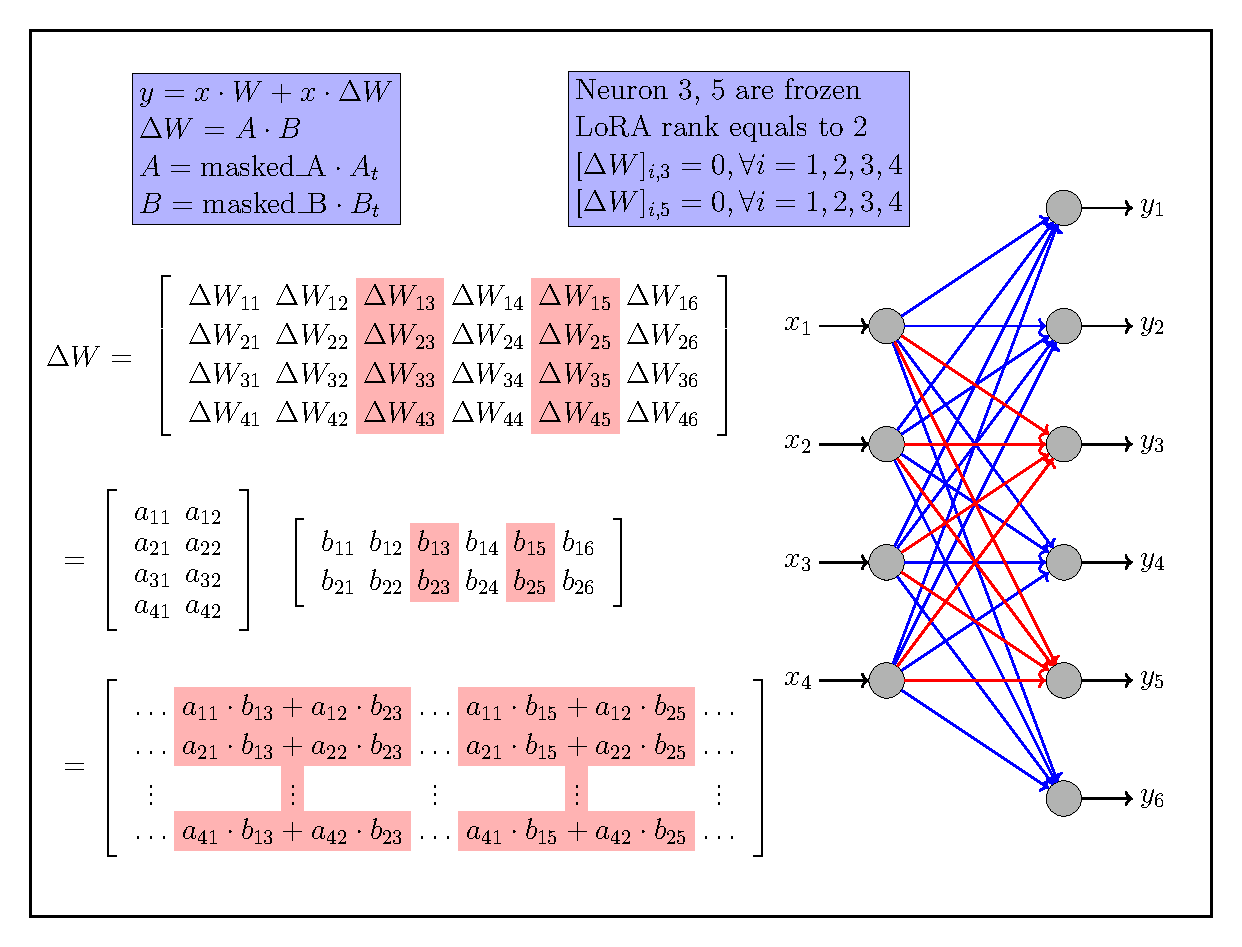
\includegraphics[width=\textwidth]{Chapters/Chapter_3/lora.pdf} % Adjust the width as needed
	\caption{LoRA fine tuning method for target neurons.}
	\label{fig:lora}
\end{figure}






